

\begin{figure}[h!]
    \centering
    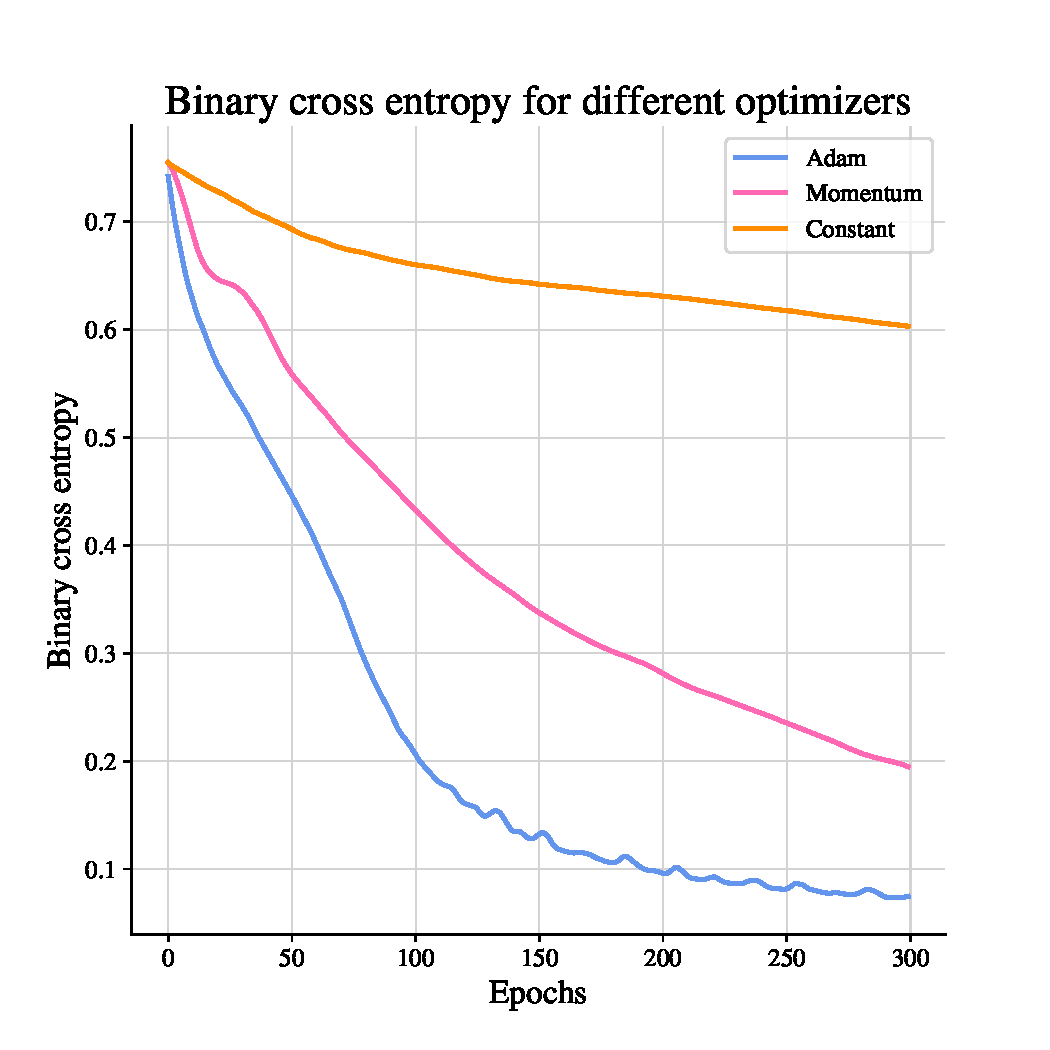
\includegraphics[width=1.0\linewidth]{project_2/figures/Binary Cross Entropy for different optimizers_classification.pdf}
    \caption{Caption}
    \label{fig:enter-label}
\end{figure}

Compare the results from the last project with the FFNN for regression tasks (can use Franke function)

Compare the results from a logistic regression with the FFNN for classification tasks (breast cancer data)

\mia{Desired plots:
\begin{itemize}
    \item Compare the gradient descent methods for OLS
    \item Compare the gradient descent methods for Ridge
    \item Compare results from FFNN to project 1 for OLS
    \item Compare results from FFNN to project 1 for Ridge
    \item compare logreg to ffnn for OLS and Ridge
\end{itemize}}

\mia{Needs discussion:\begin{itemize}
    \item Learning rate $\eta$
    \item Number of mini-batches 
    \item Number of epochs 
    \item For Ridge: the results as functions of $\lambda$
    \item lin reg code from project 1 versus ffnn
    \item critical discussion of pros and cons for each of the methods 
\end{itemize}}

